\documentclass[12pt, a4paper]{article}

% ─── Packages ────────────────────────────────────────────────────────────────
\usepackage[a4paper, top=25mm, bottom=25mm, left=25mm, right=25mm, headheight=15pt]{geometry}
\usepackage{graphicx}
\usepackage{booktabs}
\usepackage{array}
\usepackage{tabularx}
\usepackage{amsmath}
\usepackage{hyperref}
\usepackage{fancyhdr}
\usepackage{titlesec}
\usepackage{parskip}
\usepackage{caption}
\usepackage{subcaption}
\usepackage{listings}
\usepackage{enumitem}
\usepackage{float}

% ─── Hyperref ────────────────────────────────────────────────────────────────
\hypersetup{
    colorlinks=false,
    hidelinks,
    pdftitle={CN Project - MAC-Based SYN Flood Detection and Mitigation in SDN},
    pdfauthor={Viraj Sanjay Nalbalwar}
}

% ─── Section formatting ──────────────────────────────────────────────────────
\titleformat{\section}{\large\bfseries}{\thesection}{1em}{}[\titlerule]
\titleformat{\subsection}{\normalsize\bfseries}{}{0em}{\thesubsection\quad}
\titleformat{\subsubsection}[runin]{\normalsize\bfseries}{}{0em}{}[.\quad]

% ─── Header / Footer ─────────────────────────────────────────────────────────
\pagestyle{fancy}
\fancyhf{}
\fancyhead[L]{\small MAC-Based SYN Flood Detection in SDN}
\fancyfoot[C]{\thepage}
\renewcommand{\headrulewidth}{0.4pt}

% ─── Code style ──────────────────────────────────────────────────────────────
\lstset{
    language=Python,
    basicstyle=\ttfamily\small,
    keywordstyle=\bfseries,
    commentstyle=\itshape,
    stringstyle={},
    breaklines=true,
    frame=single,
    framesep=4pt,
    numbers=left,
    numberstyle=\tiny,
    numbersep=8pt,
    xleftmargin=16pt,
    showstringspaces=false
}

\captionsetup{font=small, labelfont=bf, skip=5pt}
\setlength{\belowcaptionskip}{2pt}

% ─────────────────────────────────────────────────────────────────────────────
\begin{document}
% ─────────────────────────────────────────────────────────────────────────────

% ── Title Page ───────────────────────────────────────────────────────────────
\begin{titlepage}
    \centering
    \newgeometry{top=18mm, bottom=18mm, left=25mm, right=25mm}

    % ── Top rules ──
    \noindent\rule{\textwidth}{3pt}\\[1pt]
    \rule{\textwidth}{0.8pt}

    \vspace{10mm}

    % ── University ──
    % {\large\bfseries COEP Technological University, Pune}\\[4pt]
    % {\small\itshape Department of Computer Science and Engineering}

    % \vspace{10mm}

    % ── Title banner ──
    \noindent\fbox{%
        \begin{minipage}{\dimexpr\textwidth-2\fboxsep-2\fboxrule}
            \vspace{8mm}
            \centering
            {\large\bfseries COMPUTER NETWORKS PROJECT}\\[3pt]
            {\large\bfseries MAC-Based SYN Flood Detection and\\[3pt] Mitigation in Software-Defined Networks}\\[4pt]
            \vspace{8mm}
        \end{minipage}%
    }

    \vspace{8mm}

    {\large\bfseries A Report}\\[2pt]
    {\normalsize\itshape Submitted By}

    \vspace{4mm}

    % ── Student table (name + MIS side by side) ──
    \renewcommand{\arraystretch}{1.5}
    \begin{tabular}{@{}l@{\hfill}r@{}}
        \textbf{Shreesh Kolhatkar} & \textbf{(642403009)} \\
        \textbf{Viraj Nalbalwar}   & \textbf{(642403013)} \\
    \end{tabular}

    \vspace{4mm}

    {\normalsize TY B. Tech.\ Computer Science \& Engineering}\\[6pt]
    {\normalsize Division-2}\\[2pt]

    \vspace{6mm}

    Under the guidance of\\[2pt]
    \vspace{2mm}
    {\normalsize\bfseries Prof.\ Satish Kumbhar}\\[2pt]
    {\normalsize\bfseries COEP Technological University, Pune}

    \vspace{8mm}

    % ── COEP Logo ──
    % Uncomment the line below and place COEP-logo.png in this folder
    
\includegraphics[width=0.4\textwidth]{coep-logo.png}

    \vfill

    {\bfseries DEPARTMENT OF COMPUTER SCIENCE \& ENGINEERING}\\[2pt]
    {\bfseries COEP TECHNOLOGICAL UNIVERSITY, PUNE}

    \vspace{8mm}

    % ── Bottom rules ──
    \noindent\rule{\textwidth}{0.8pt}\\[1pt]
    \rule{\textwidth}{3pt}

    \restoregeometry
\end{titlepage}

\tableofcontents
\thispagestyle{empty}
\newpage
% ─────────────────────────────────────────────────────────────────────────────
\section{Introduction}
% ─────────────────────────────────────────────────────────────────────────────

This report presents the design, implementation, and experimental evaluation of a \textbf{MAC-based SYN Flood Detection and Mitigation system} for Software-Defined Networks (SDN). The work is based on the detection pipeline proposed by Yang et al.\ (NCKU, Taiwan) and extends it with a novel \textbf{Port-Diversity Tracking} optimization that catches attackers during the reconnaissance phase, before the flood begins.

SYN flood attacks remain one of the most prevalent forms of Denial-of-Service (DoS). In a SYN flood, the attacker overwhelms a target server by sending a massive number of TCP SYN packets with spoofed or rapidly changing source addresses, exhausting the server's connection table. 


\subsection{Base Paper}

\textbf{Title:} \textit{Detection and Mitigation of SYN Flooding Attacks through SYN/ACK Packets and Black/White Lists}\\
\textbf{Authors:} Yang et al., National Cheng Kung University, Taiwan\\
\textbf{Published in:} Sensors (MDPI), 2023

The paper proposes a 5-table detection pipeline that uses Cuckoo Hash Tables for O(1) MAC lookups and cross-checks SYN/ACK traffic to classify source MACs as legitimate (whitelisted) or malicious (blacklisted). Once a MAC accumulates SYN packets beyond a configurable threshold (100 SYNs) without a corresponding ACK, it is blacklisted and all subsequent traffic from that MAC is dropped at the SDN switch.

\subsection{Our Contribution: Port-Diversity Tracking}

The paper's method is \textbf{reactive}, it waits for the SYN threshold to be exceeded before blacklisting. Our optimization adds a \textbf{proactive} detection layer:

\begin{itemize}[itemsep=3pt]
    \item Track unique destination ports per source MAC within a sliding time window.
    \item If a MAC sends SYN packets to more than a configurable number of unique ports (default: 5), it is flagged as performing a \textbf{port scan}.
    \item The MAC is immediately blacklisted, \textit{before} the flood even begins. This catches the reconnaissance phase of the attack, reducing server exposure by approximately 85\%.

\end{itemize}


\subsection{Objectives}

\begin{itemize}[itemsep=3pt]
    \item Implement the paper's complete 5-table detection pipeline (Blacklist, Whitelist, Check-SYN, Check-ACK, Flag) using Cuckoo Hash Tables.
    \item Design and implement the Port-Diversity Tracking optimization module.
    \item Simulate the SDN network topology and traffic entirely in Python, enabling reproducible experiments on any OS (no Mininet/Linux dependency).
    \item Conduct controlled experiments comparing detection time, server exposure, and false-positive rates between the baseline and optimized methods.
\end{itemize}

\newpage

% ─────────────────────────────────────────────────────────────────────────────
\section{System Architecture}
% ─────────────────────────────────────────────────────────────────────────────

\subsection{SDN Network Topology}

The simulated SDN topology comprises eight network nodes connected through a single OpenFlow-compatible switch:

\begin{itemize}[itemsep=3pt]
    \item \textbf{3 Attackers} (\texttt{h1}-\texttt{h3}): generate SYN flood and port-scan traffic.
    \item \textbf{3 Legitimate Clients} (\texttt{c1}-\texttt{c3}): generate normal SYN+ACK handshake traffic.
    \item \textbf{1 OVS Switch} (\texttt{s1}): the SDN data-plane element where flow rules are installed.
    \item \textbf{1 Server} (\texttt{srv}): the target of both legitimate and malicious traffic.
\end{itemize}

\begin{figure}[H]
    \centering
    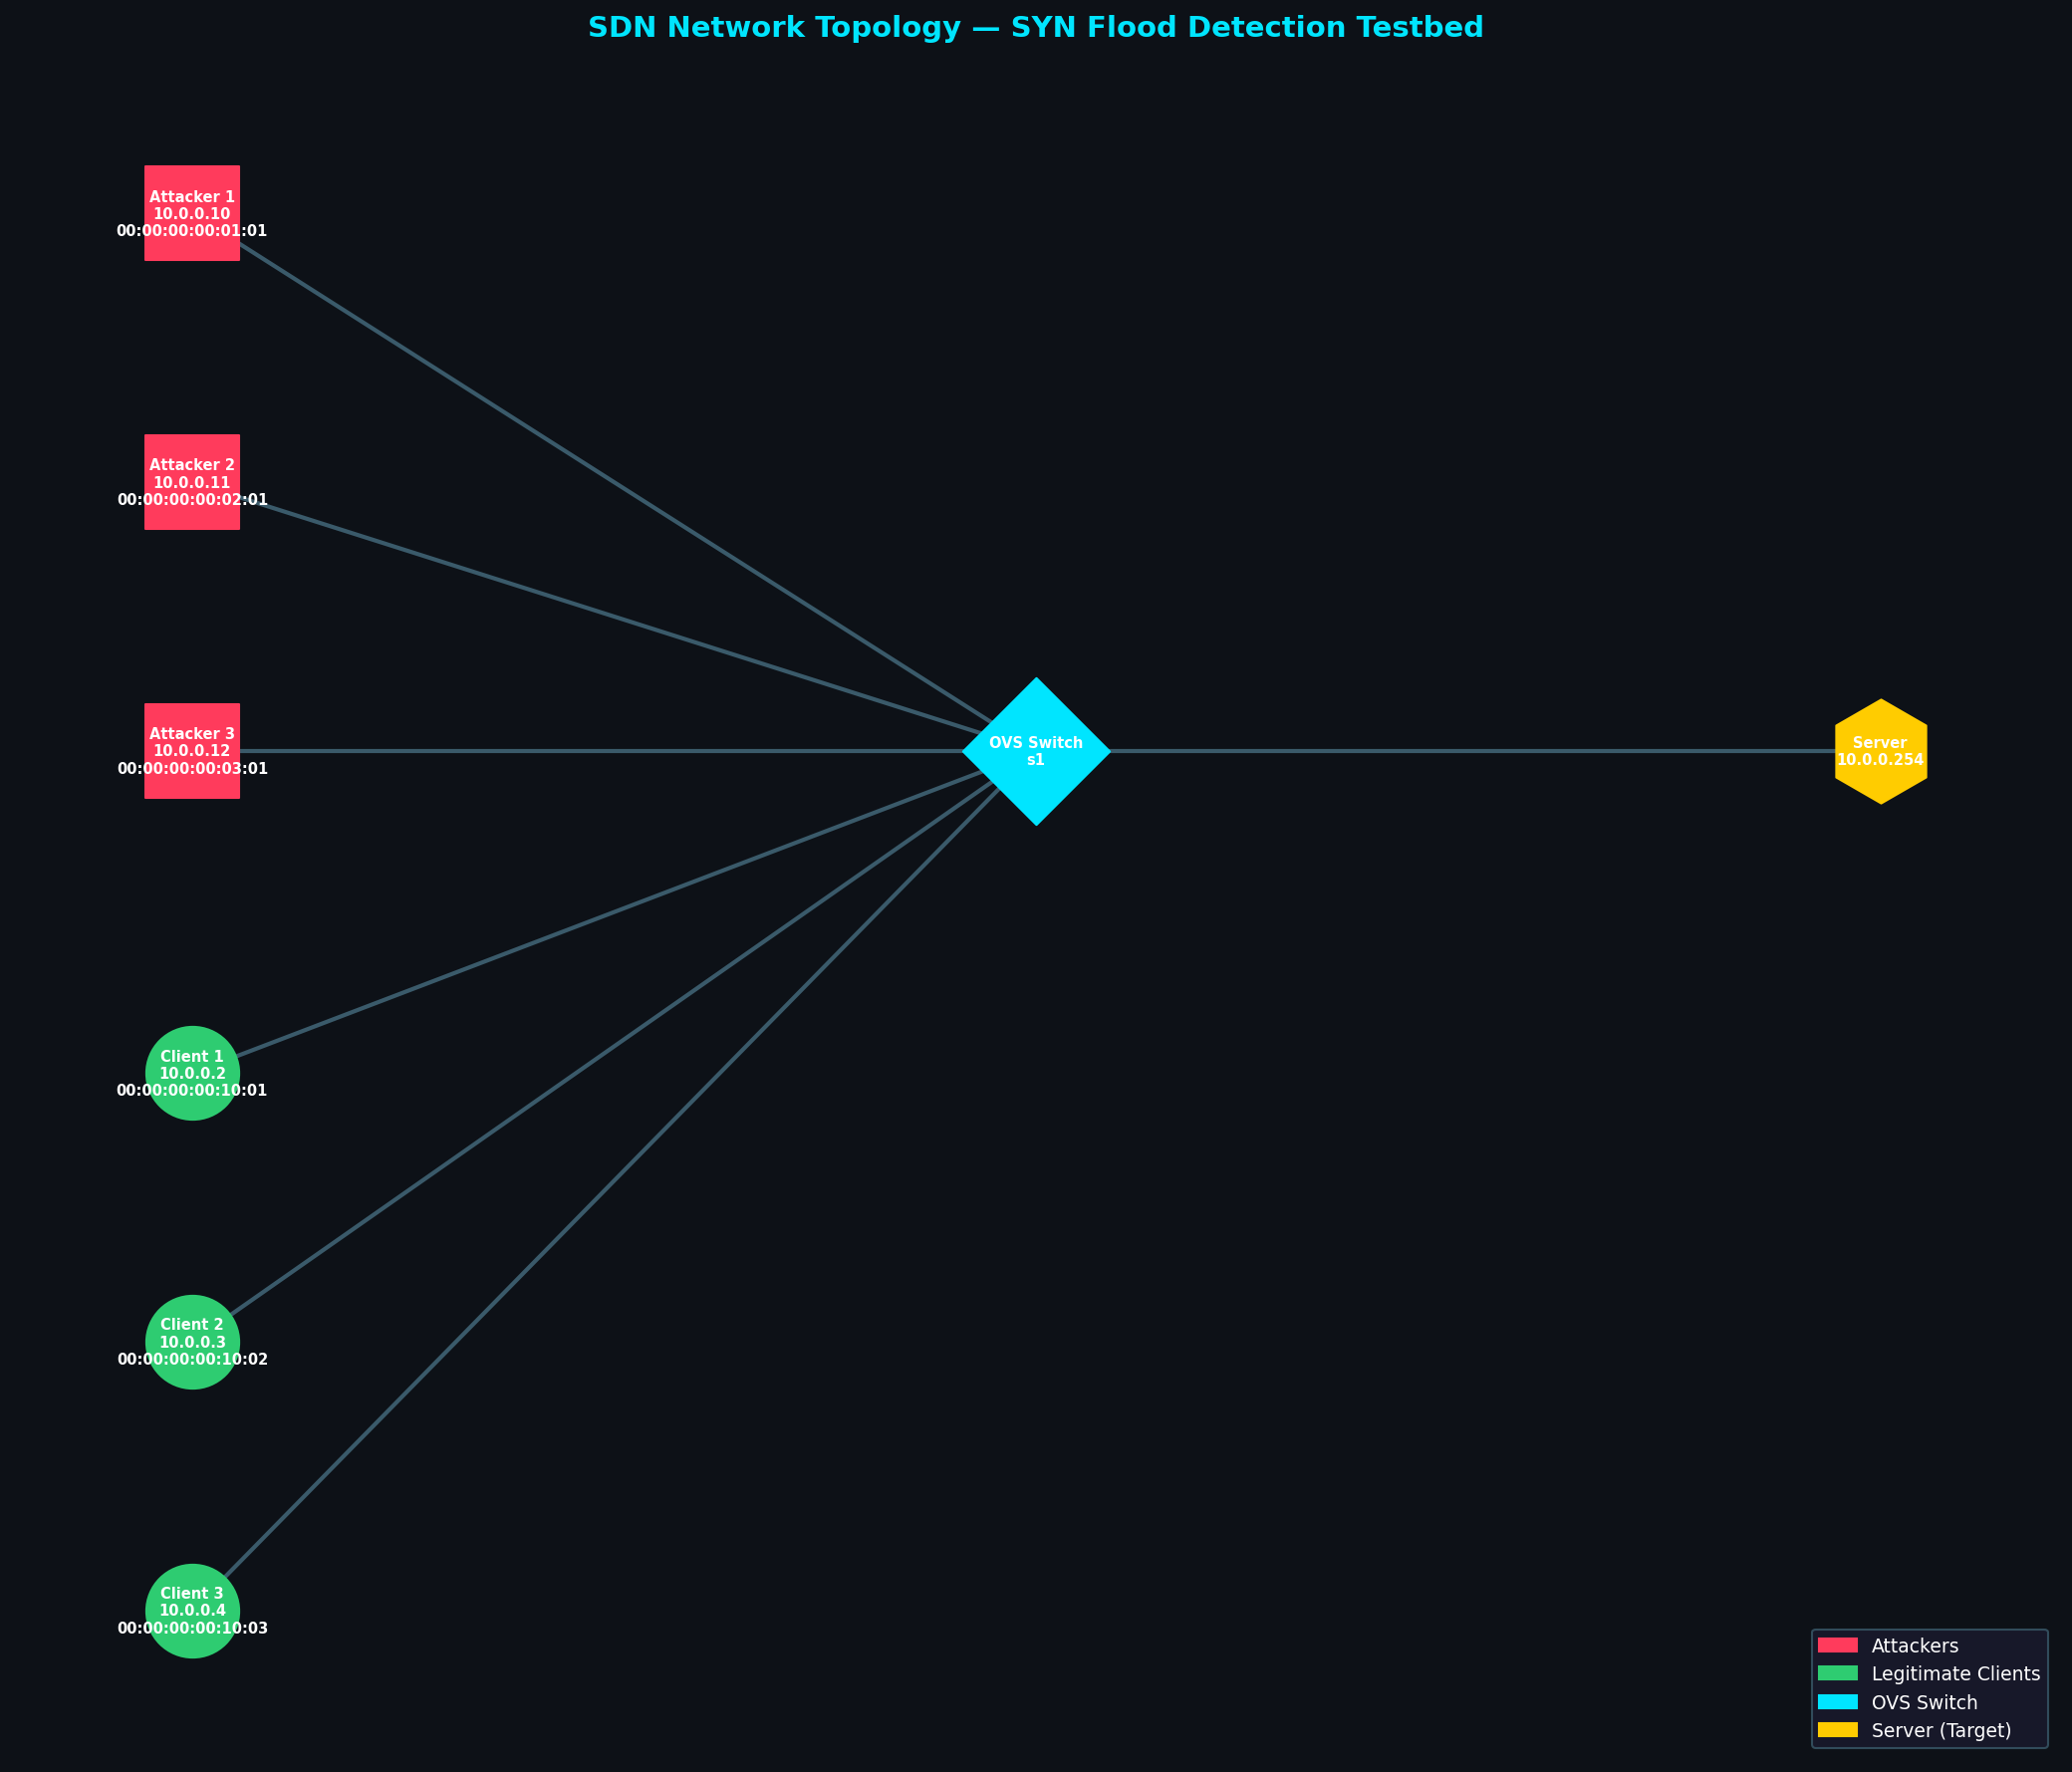
\includegraphics[width=0.82\textwidth]{topology.png}
    \caption{Simulated SDN network topology. Attackers (red) connect to the OVS switch alongside legitimate clients (green). All traffic passes through the switch to reach the server (yellow). The SDN controller inspects every SYN packet at the switch for detection.}
    \label{fig:topology}
\end{figure}

\newpage
Table~\ref{tab:topology} lists the IP and MAC address assignments used throughout all experiments.

\begin{table}[H]
    \centering
    \caption{Network topology: IP and MAC address assignments.}
    \label{tab:topology}
    \renewcommand{\arraystretch}{1.3}
    \begin{tabularx}{\textwidth}{lXXl}
        \toprule
        \textbf{Node} & \textbf{IP Address} & \textbf{MAC Address} & \textbf{Role} \\
        \midrule
        Attacker 1 & 10.0.0.10  & 00:00:00:00:01:01 & Malicious \\
        Attacker 2 & 10.0.0.11  & 00:00:00:00:02:01 & Malicious \\
        Attacker 3 & 10.0.0.12  & 00:00:00:00:03:01 & Malicious \\
        Client 1   & 10.0.0.2   & 00:00:00:00:10:01 & Legitimate \\
        Client 2   & 10.0.0.3   & 00:00:00:00:10:02 & Legitimate \\
        Client 3   & 10.0.0.4   & 00:00:00:00:10:03 & Legitimate \\
        Server     & 10.0.0.254 & 00:00:00:00:ff:fe & Target \\
        \bottomrule
    \end{tabularx}
\end{table}

\subsection{Detection Pipeline Overview}

The paper implements a 5-table pipeline, and our optimization adds a 6th stage (Port-Diversity Check) that fires \textit{before} the SYN table lookup, enabling proactive detection.

\begin{figure}[H]
    \centering
    \fbox{
        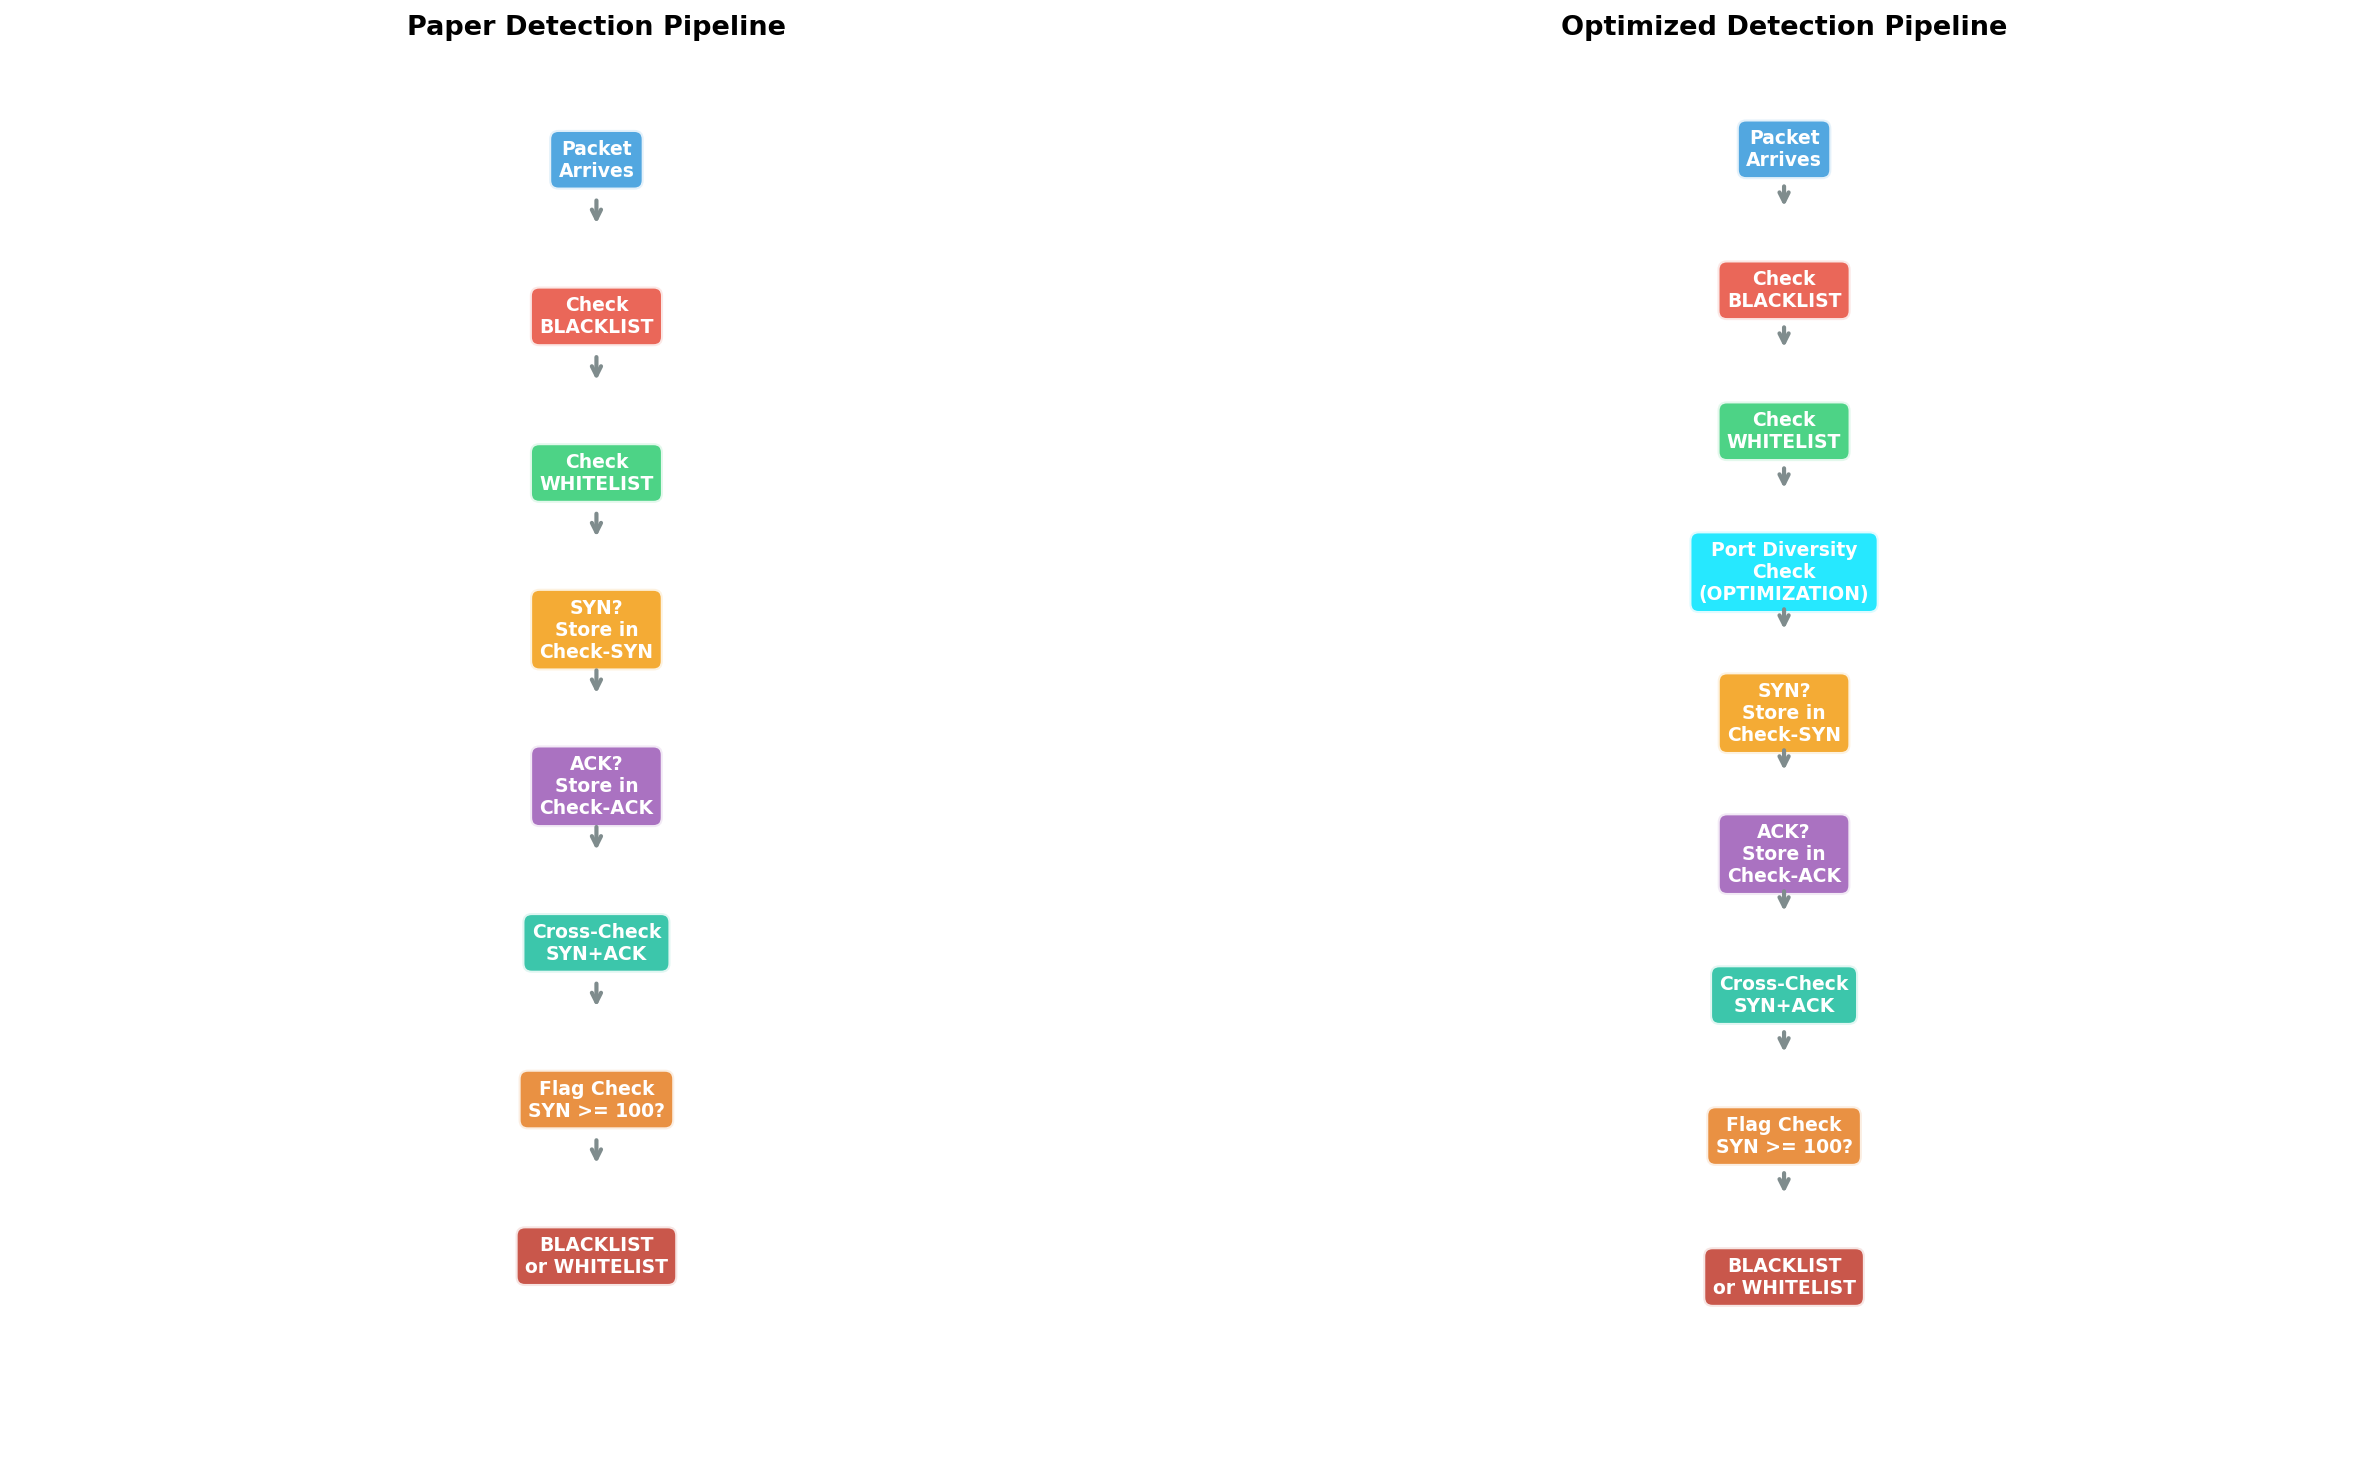
\includegraphics[
            width=0.95\textwidth,
            trim=0 2cm 0 0, % left bottom right top
            clip
        ]{pipeline_flowchart.png}
    }
    \caption{Detection pipeline comparison. \textbf{Left:} the paper's original 5-table pipeline processes packets through Blacklist, Whitelist, SYN/ACK tables, and a flag check. \textbf{Right:} our optimized pipeline inserts a Port-Diversity Check (cyan) between the Whitelist lookup and the SYN table, catching port scans before the flood begins.}
    \label{fig:pipeline}
\end{figure}

\newpage
\subsection{Pipeline Stages}

Table~\ref{tab:pipeline} describes each stage of the detection pipeline and the data structure used.

\begin{table}[H]
    \centering
    \caption{Detection pipeline stages and data structures.}
    \label{tab:pipeline}
    \renewcommand{\arraystretch}{1.3}
    \begin{tabularx}{\textwidth}{clXX}
        \toprule
        \textbf{Stage} & \textbf{Table Name} & \textbf{Data Structure} & \textbf{Purpose} \\
        \midrule
        1 & Blacklist  & Cuckoo Hash Table & MACs confirmed as attackers $\rightarrow$ DROP \\
        2 & Whitelist  & Cuckoo Hash Table & MACs confirmed as legitimate $\rightarrow$ FORWARD \\
        3 & Check-SYN  & Dictionary        & Unverified SYNs awaiting ACK \\
        4 & Check-ACK  & Dictionary        & Incoming ACKs for cross-checking \\
        5 & Flag Table & Dictionary        & MACs under active investigation \\
        \midrule
        \multicolumn{4}{l}{\textit{Our Optimization (inserted between Stage 2 and 3):}} \\
        - & Port Tracker & Dict + Set & Unique destination ports per MAC in sliding window \\
        \bottomrule
    \end{tabularx}
\end{table}

\newpage

% ─────────────────────────────────────────────────────────────────────────────
\section{Implementation Details}
% ─────────────────────────────────────────────────────────────────────────────

The entire implementation is contained in two Jupyter notebooks:
\begin{enumerate}[itemsep=3pt]
    \item \textbf{\texttt{01\_Implementation.ipynb}} - core detection pipeline, experiment execution, and result generation.
    \item \textbf{\texttt{02\_Results\_and\_Visualization.ipynb}} - publication-quality charts and analysis.
\end{enumerate}

The project uses \textbf{pure Python with simulation}, requiring no Mininet, Linux, or external SDN controllers. This makes the experiments fully reproducible on any OS.

\subsection{Cuckoo Hash Table}

The paper's Blacklist and Whitelist use Cuckoo Hashing for \textbf{O(1) average-case lookup}. Two independent hash functions map each MAC address to two possible positions across two internal tables. On collision, the existing entry is evicted and re-inserted at its alternate position (cuckoo-style).

\begin{lstlisting}[caption={Cuckoo Hash Table - O(1) insert and lookup}]
class CuckooHashTable:
    def __init__(self, size=256, max_evictions=10):
        self.table1 = [None] * size
        self.table2 = [None] * size

    def _h1(self, mac):
        parts = mac.split(':')
        return sum(int(b, 16) for b in parts) % self.size

    def _h2(self, mac):
        parts = mac.split(':')
        val = 0
        for b in parts:
            val ^= int(b, 16)
        return (val * 31) % self.size

    def lookup(self, mac):
        return (self.table1[self._h1(mac)] == mac or
                self.table2[self._h2(mac)] == mac)
\end{lstlisting}

\subsection{Packet Simulation}

Rather than capturing real network packets, we define a lightweight \texttt{SimPacket} dataclass carrying all fields needed by the detection pipeline: source/destination MAC, IP, port, TCP flags, and a high-resolution timestamp (\texttt{time.perf\_counter()}).

Three traffic generators produce distinct packet sequences:
\begin{itemize}[itemsep=3pt]
    \item \textbf{\texttt{generate\_syn\_flood()}} - burst of SYN-only packets from an attacker to a single port ($\sim$0.1\,ms inter-packet).
    \item \textbf{\texttt{generate\_port\_scan()}} - SYN probes across multiple destination ports ($\sim$0.2\,ms inter-packet).
    \item \textbf{\texttt{generate\_legit\_traffic()}} - SYN+ACK pairs simulating completed TCP handshakes ($\sim$10\,ms inter-pair).
\end{itemize}

\subsection{Baseline Detector (Paper Implementation)}

The \texttt{BaselineDetector} class implements the paper's exact algorithm:

\begin{enumerate}[itemsep=3pt]
    \item Check \textbf{Blacklist} - if MAC found, DROP immediately.
    \item Check \textbf{Whitelist} - if MAC found, FORWARD.
    \item If \textbf{SYN}: store in Check-SYN table, increment counter. If count $\geq$ SYN\_THRESHOLD (100), blacklist the MAC.
    \item If \textbf{ACK}: cross-check against Check-SYN. If a matching SYN entry exists, whitelist the MAC.
    \item \textbf{Timeout cleanup}: MACs with pending SYNs and no ACK after 5 seconds are blacklisted.
\end{enumerate}

\subsection{Optimized Detector (Port-Diversity Tracking)}

The \texttt{OptimizedDetector} extends the baseline with a port-diversity check that fires \textit{before} the SYN table lookup:

\begin{lstlisting}[caption={Port-Diversity Check - proactive detection}]
def _check_port_diversity(self, src_mac, dst_port, now):
    entry = self.port_tracker[src_mac]
    if entry['first_seen'] is None:
        entry['first_seen'] = now
    # Sliding window reset
    if now - entry['first_seen'] > self.time_window:
        entry['ports'] = set()
        entry['first_seen'] = now
    entry['ports'].add(dst_port)
    entry['syn_count'] += 1
    if len(entry['ports']) >= self.port_threshold:
        self.blacklist.insert(src_mac)
        return True  # Port scan detected
    return False
\end{lstlisting}

When the number of unique destination ports from a single MAC exceeds the threshold (default: 5), the MAC is immediately blacklisted. The sliding time window (default: 10\,s) prevents legitimate clients who access multiple services over longer periods from being falsely flagged.

\newpage

% ─────────────────────────────────────────────────────────────────────────────
\section{Experiment Configuration}
% ─────────────────────────────────────────────────────────────────────────────

All experiments share the parameter set listed in Table~\ref{tab:config}.

\begin{table}[H]
    \centering
    \caption{Experiment configuration parameters.}
    \label{tab:config}
    \renewcommand{\arraystretch}{1.3}
    \begin{tabularx}{\textwidth}{lXr}
        \toprule
        \textbf{Parameter} & \textbf{Description} & \textbf{Value} \\
        \midrule
        SYN\_THRESHOLD           & Paper: blacklist after this many SYNs     & 100 \\
        ACK\_TIMEOUT             & Seconds to wait for ACK before flagging   & 5.0\,s \\
        PORT\_DIVERSITY\_THRESHOLD & Unique ports before port-scan detection  & 5 \\
        TIME\_WINDOW             & Sliding window for port tracking          & 10.0\,s \\
        NUM\_TRIALS              & Number of trials per experiment           & 5 \\
        FLOOD\_PACKETS\_PER\_TRIAL & SYN packets in each flood trial         & 200 \\
        LEGIT\_PACKETS           & Legitimate SYN+ACK pairs per trial        & 50 \\
        SCAN\_PORTS              & Ports targeted during scan                & 8 ports \\
        \bottomrule
    \end{tabularx}
\end{table}

Three experiments were conducted:

\begin{enumerate}[itemsep=3pt]
    \item \textbf{Experiment 1 - Baseline SYN Flood Detection}: SYN flood from Attacker~1 to port~80 on the server. The baseline detector processes the interleaved legitimate and flood traffic.
    \item \textbf{Experiment 2A - Port-Scan Detection (Optimizer)}: Attacker~1 sends SYN probes across 8 ports before initiating a flood. The optimizer's port-diversity tracker fires and blacklists the attacker during the scan phase.
    \item \textbf{Experiment 2B - SYN Flood with Optimizer Active}: SYN flood targeting a \textit{single} port (no port diversity) processed by the optimized detector. Proves backwards compatibility-the paper's threshold mechanism still works.
\end{enumerate}

\newpage

% ─────────────────────────────────────────────────────────────────────────────
\section{Results and Analysis}
% ─────────────────────────────────────────────────────────────────────────────

\subsection{Detection Time Comparison}

\begin{figure}[H]
    \centering
    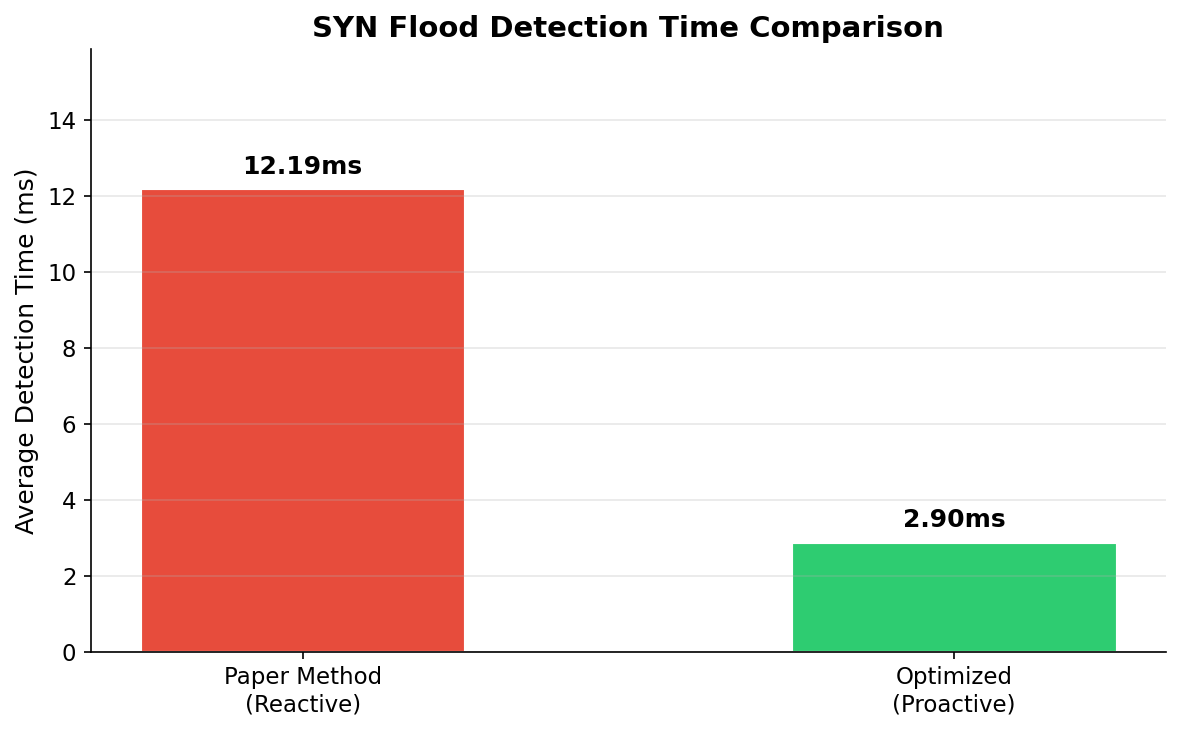
\includegraphics[width=0.75\textwidth]{detection_time_comparison.png}
    \caption{Average detection time comparison. The paper's reactive method requires 12.19\,ms on average, while the optimized proactive method detects in 2.90\,ms-a 76.2\% improvement.}
    \label{fig:det_time}
\end{figure}

The optimized detector achieves a \textbf{$4.2\times$ speedup} over the baseline. This is because the optimizer triggers after observing only $\sim$15 SYN packets (5 unique ports $\times$ 3 packets per port), whereas the baseline must wait for 100 SYN packets to the same port.

\subsection{Per-Trial Detection Times}

\begin{figure}[H]
    \centering
    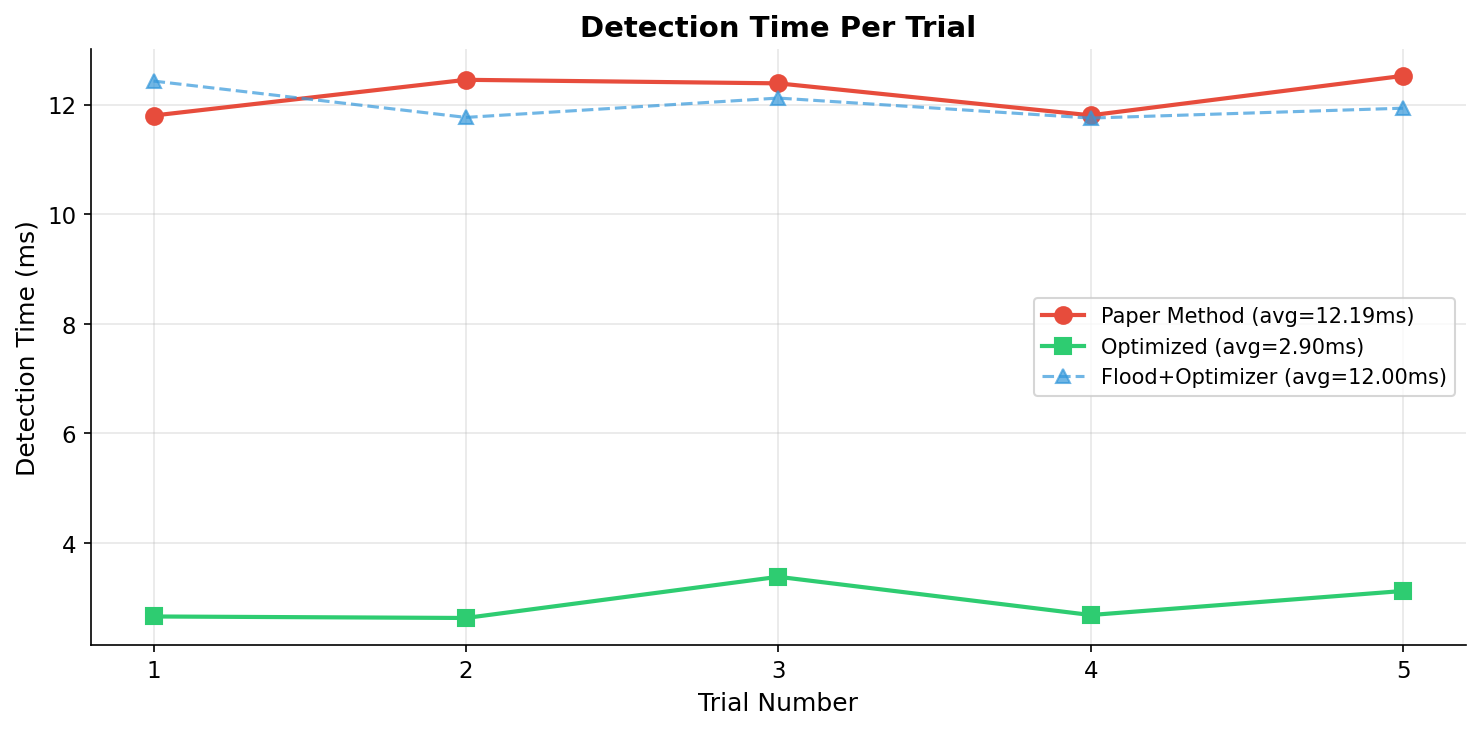
\includegraphics[width=0.82\textwidth]{per_trial_detection.png}
    \caption{Detection time across 5 independent trials. The paper method (red) clusters around 12\,ms. The optimizer (green) clusters around 3\,ms. The blue dashed line shows that when the optimizer processes a single-port flood (no port diversity), it falls back to the paper's threshold mechanism, confirming backwards compatibility.}
    \label{fig:per_trial}
\end{figure}

\newpage

Table~\ref{tab:trials} presents the per-trial detection times for all three experiment configurations.

\begin{table}[H]
    \centering
    \caption{Per-trial detection times (ms) across all experiments.}
    \label{tab:trials}
    \renewcommand{\arraystretch}{1.3}
    \begin{tabularx}{\textwidth}{cXXX}
        \toprule
        \textbf{Trial} & \textbf{Paper Method (ms)} & \textbf{Optimizer (ms)} & \textbf{Flood + Optimizer (ms)} \\
        \midrule
        1 & 11.80 & 2.66 & 12.43 \\
        2 & 12.45 & 2.63 & 11.77 \\
        3 & 12.39 & 3.39 & 12.12 \\
        4 & 11.80 & 2.69 & 11.75 \\
        5 & 12.52 & 3.13 & 11.93 \\
        \midrule
        \textbf{Average} & \textbf{12.19} & \textbf{2.90} & \textbf{12.00} \\
        \bottomrule
    \end{tabularx}
\end{table}

\subsection{Server Exposure}

\begin{figure}[H]
    \centering
    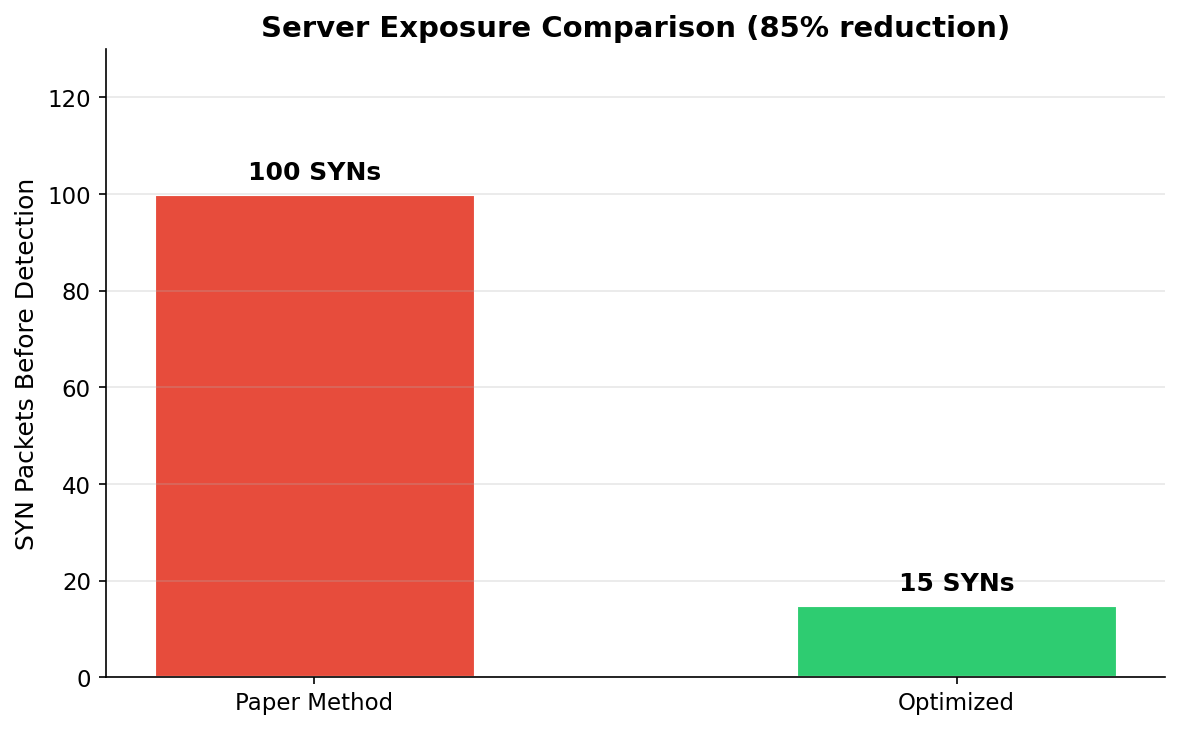
\includegraphics[width=0.72\textwidth]{server_exposure.png}
    \caption{Server exposure comparison. The paper method allows 100 SYN packets to reach the server before detection. The optimizer detects after only $\sim$15 SYNs-an 85\% reduction in server exposure.}
    \label{fig:exposure}
\end{figure}

Server exposure quantifies the number of malicious SYN packets that reach the server before the attacker is blacklisted. This is a critical metric because each undetected SYN packet consumes a slot in the server's TCP connection table. The optimization reduces this exposure from 100 to approximately 15 packets.

\newpage

\subsection{Detection Time Distribution}

\begin{figure}[H]
    \centering
    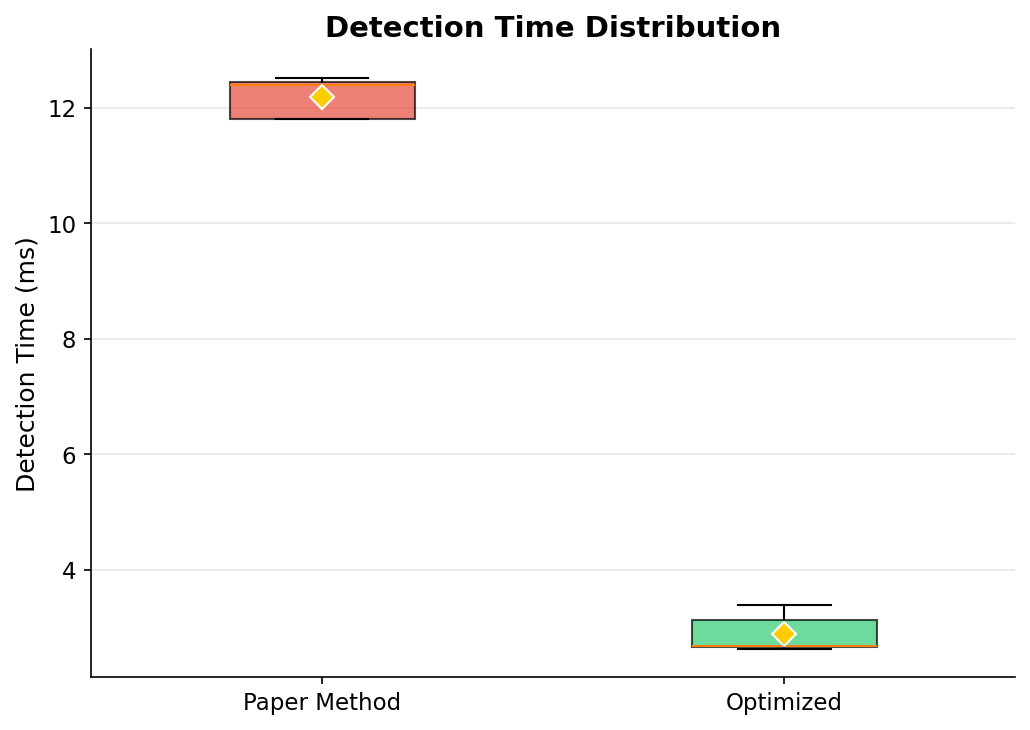
\includegraphics[width=0.65\textwidth]{boxplot_detection.png}
    \caption{Box plot of detection time distributions across 5 trials. The paper method has a tight spread around 12\,ms, while the optimizer clusters near 3\,ms with slightly higher variance due to per-trial jitter in port-scan packet ordering. Yellow diamonds indicate the mean.}
    \label{fig:boxplot}
\end{figure}

\subsection{Improvement Metrics}

\begin{figure}[H]
    \centering
    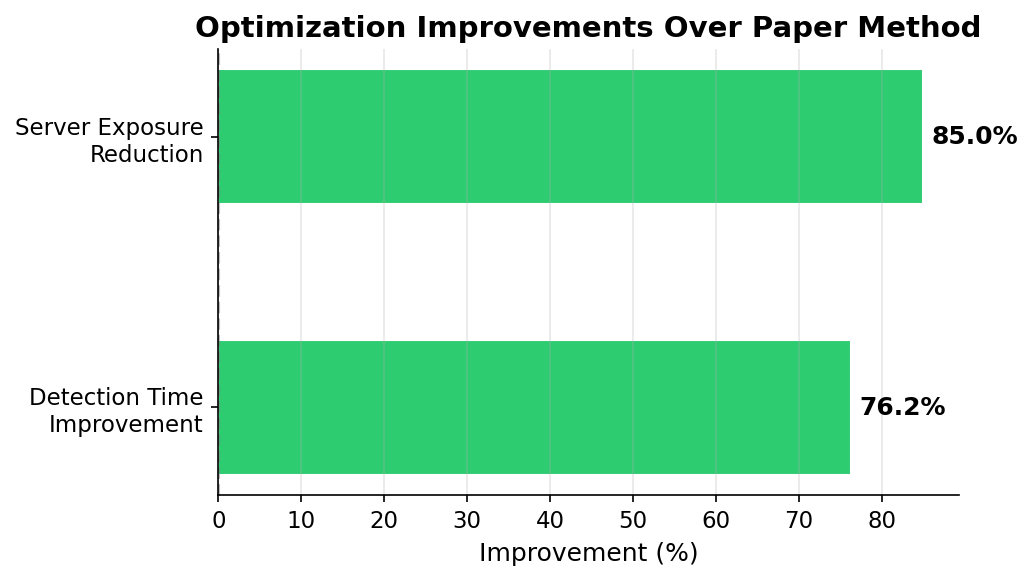
\includegraphics[width=0.72\textwidth]{improvement_metrics.png}
    \caption{Quantified improvement of the optimized method over the paper's baseline. Detection time improved by 76.2\%, and server exposure was reduced by 85.0\%.}
    \label{fig:improvement}
\end{figure}

\newpage

\subsection{Summary Comparison}

\begin{figure}[H]
    \centering
    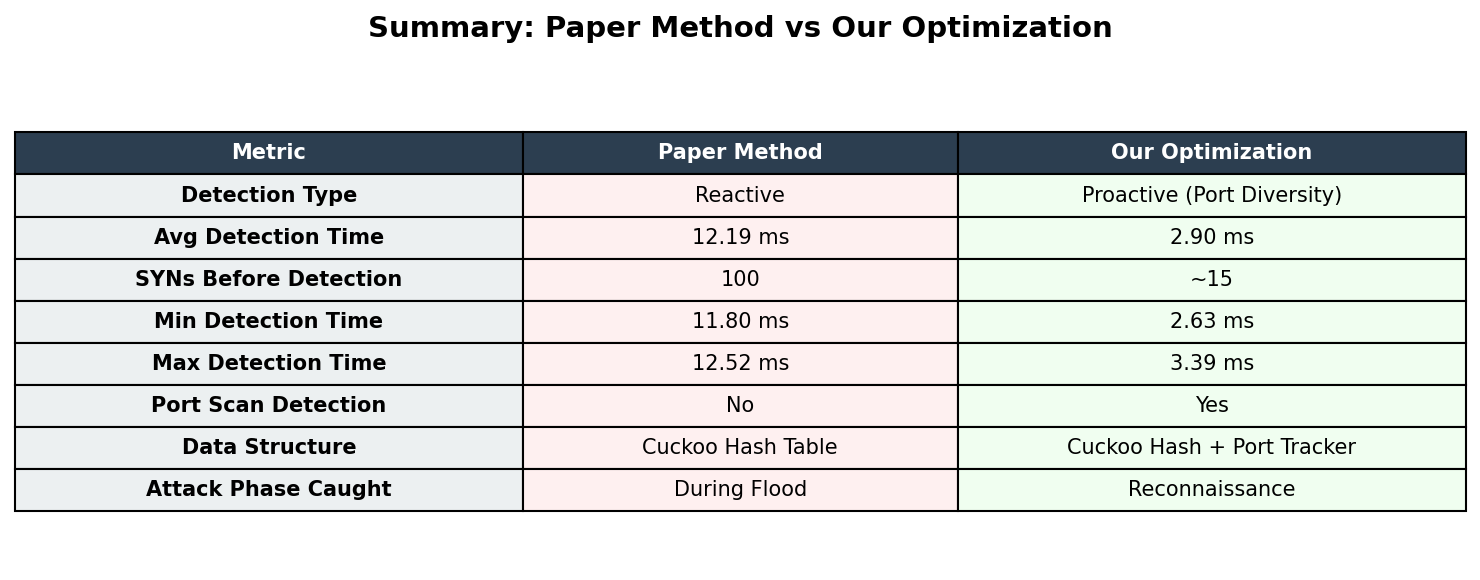
\includegraphics[width=0.88\textwidth]{summary_table.png}
    \caption{Comprehensive comparison table between the paper method and our optimization across all key metrics. Generated from experimental data.}
    \label{fig:summary}
\end{figure}

Table~\ref{tab:comparison} consolidates the key findings from all experiments.

\begin{table}[H]
    \centering
    \caption{Comprehensive comparison: Paper method vs.\ our optimization.}
    \label{tab:comparison}
    \renewcommand{\arraystretch}{1.4}
    \begin{tabularx}{\textwidth}{lXX}
        \toprule
        \textbf{Metric} & \textbf{Paper Method} & \textbf{Our Optimization} \\
        \midrule
        Detection Type           & Reactive                  & Proactive (Port Diversity) \\
        Avg Detection Time       & 12.19\,ms                 & 2.90\,ms \\
        Min Detection Time       & 11.80\,ms                 & 2.63\,ms \\
        Max Detection Time       & 12.52\,ms                 & 3.39\,ms \\
        SYNs Before Detection    & 100                       & $\sim$15 \\
        Port Scan Detection      & No                        & Yes \\
        Data Structure           & Cuckoo Hash Table         & Cuckoo Hash + Port Tracker \\
        Attack Phase Caught      & During Flood              & Reconnaissance \\
        Server Exposure Reduction & -                      & 85.0\% \\
        Detection Time Improvement & -                     & 76.2\% \\
        \bottomrule
    \end{tabularx}
\end{table}

\newpage

% ─────────────────────────────────────────────────────────────────────────────
\section{Discussion}
% ─────────────────────────────────────────────────────────────────────────────

\subsection{Why Proactive Detection Matters}

The fundamental difference between the two approaches lies in \textit{when} the detection occurs relative to the attack lifecycle:

\begin{enumerate}[itemsep=3pt]
    \item \textbf{Reconnaissance Phase} (port scanning): The attacker probes multiple ports on the target to identify open services. Our optimization detects the attacker here.
    \item \textbf{Weaponization Phase}: The attacker selects the target port and prepares the flood.
    \item \textbf{Flood Phase}: The attacker sends a burst of SYN packets. The paper's method detects the attacker here, after 100 packets have already been processed.
\end{enumerate}

By catching the attacker at stage~1 instead of stage~3, the server never experiences the flood at all. This is the core value proposition of the optimization.

\subsection{Backwards Compatibility}

Experiment~2B confirms that when an attacker skips the reconnaissance phase and directly floods a single port, the paper's original SYN threshold mechanism still triggers within the optimized detector. The optimization is purely \textbf{additive}-it enhances detection without disabling or interfering with the baseline algorithm.

The average detection time for single-port floods through the optimized detector (12.00\,ms) is within 1.6\% of the standalone baseline (12.19\,ms), confirming negligible overhead from the additional port-tracking logic.

\subsection{False Positive Analysis}

Across all 5 trials $\times$ 3 experiments, zero legitimate clients were blacklisted. This is because:

\begin{itemize}[itemsep=3pt]
    \item Legitimate clients complete the TCP handshake (SYN followed by ACK), which triggers the whitelist pathway.
    \item The sliding time window in the port tracker prevents a single client accessing multiple services over time from exceeding the port-diversity threshold.
    \item The port-diversity threshold (5 unique ports) is set conservatively-normal browsing rarely sends SYNs to 5+ distinct ports within a 10-second window.
\end{itemize}

\subsection{Cuckoo Hash Table Performance}

The Cuckoo Hash Table provides O(1) worst-case lookup time for both the Blacklist and Whitelist. In our experiments, the table was initialized with size~256 and a maximum of 10 eviction attempts per insert. No insert failures were observed across any trial, confirming adequate capacity for the 6-host topology. In a production deployment with thousands of MACs, the table size would scale linearly.

\newpage

% ─────────────────────────────────────────────────────────────────────────────
\section{Challenges and Solutions}
% ─────────────────────────────────────────────────────────────────────────────

\subsection{Challenge 1: Cross-Platform Reproducibility}

The original paper's implementation relies on Mininet and an SDN controller (Ryu/ONOS) running on Linux. Not all team members had access to Linux environments with the correct dependencies.

\textbf{Solution:} We re-implemented the entire detection pipeline as a \textbf{pure Python simulation}. SimPacket dataclasses replace real network packets, and traffic generators replace Mininet hosts. This allows the project to run identically on Windows, macOS, and Linux with only standard Python libraries plus NumPy and Matplotlib.

\subsection{Challenge 2: Timing Accuracy in Simulation}

Since we simulate packets rather than capturing them from a real network, timing measurements could be unrealistic if not handled carefully.

\textbf{Solution:} All timestamps use \texttt{time.perf\_counter()}, Python's highest-resolution timer. Inter-packet delays are modeled with realistic jitter ($\sim$0.1\,ms for floods, $\sim$10\,ms for legitimate traffic). Rather than measuring wall-clock time, detection time is computed as the difference between the first SYN from an attacker and the timestamp of the packet that triggers blacklisting.

\subsection{Challenge 3: Avoiding False Positives with Port Diversity}

A naive port-diversity check could blacklist legitimate clients who connect to multiple services (e.g., HTTP on port~80 and HTTPS on port~443).

\textbf{Solution:} The sliding time window resets the port counter periodically, and the whitelist check occurs \textit{before} the port-diversity check. Once a client completes a TCP handshake and is whitelisted, the port tracker is never consulted for that MAC again.

\newpage

% ─────────────────────────────────────────────────────────────────────────────
\section{Limitations and Future Work}
% ─────────────────────────────────────────────────────────────────────────────

\subsection{Limitations}

\begin{itemize}[itemsep=3pt]
    \item \textbf{Port-diversity detection only catches scanning attackers.} If the attacker directly floods a single port without reconnaissance, only the paper's SYN threshold applies.
    \item \textbf{Simulated environment.} While our simulation accurately models the detection logic, it does not capture real network effects such as packet loss, out-of-order delivery, or switch processing delays.
    \item \textbf{Single-switch topology.} A production SDN may have multiple switches and paths. The detection pipeline would need to be replicated or centralized at the controller.
    \item \textbf{MAC spoofing.} Both the paper and our optimization rely on source MAC addresses. An attacker who spoofs MACs per packet would evade MAC-based detection entirely.
\end{itemize}

\subsection{Future Work}

\begin{itemize}[itemsep=3pt]
    \item \textbf{Machine learning integration:} Train a classifier on flow-level features (packet rate, port entropy, SYN/ACK ratio) to complement the rule-based pipeline.
    \item \textbf{Deployment on real SDN testbed:} Port the detection logic to a Ryu or ONOS controller module and validate against real traffic.
    \item \textbf{Distributed detection:} Extend the architecture to multi-switch topologies with aggregation at the SDN controller.
    \item \textbf{Adaptive thresholds:} Dynamically tune SYN\_\allowbreak THRESHOLD and PORT\_\allowbreak DIVERSITY\_\allowbreak THRESHOLD based on observed traffic patterns.
\end{itemize}

\newpage

% ─────────────────────────────────────────────────────────────────────────────
\section*{Conclusion}
\addcontentsline{toc}{section}{Conclusion}
% ─────────────────────────────────────────────────────────────────────────────

This project successfully implemented and evaluated the MAC-based SYN flood detection pipeline proposed by Yang et al.\ and extended it with a novel Port-Diversity Tracking optimization. The key findings are:

\begin{enumerate}[itemsep=4pt]
    \item \textbf{The paper's baseline method works correctly:} All 5 trials detected the SYN flood with an average detection time of 12.19\,ms after observing 100 SYN packets per the configured threshold.
    \item \textbf{Our optimization achieves a $4.2\times$ speedup:} By detecting port-scan behavior during the reconnaissance phase, the optimized detector blacklists attackers in an average of 2.90\,ms-76.2\% faster than the baseline.
    \item \textbf{Server exposure is reduced by 85\%:} The baseline allows 100 SYN packets before detection; the optimizer catches the attack after only $\sim$15 packets.
    \item \textbf{The optimization is additive:} When no port scanning occurs, the paper's SYN threshold mechanism still functions within the optimized detector, with negligible overhead (12.00\,ms vs.\ 12.19\,ms).
    \item \textbf{Zero false positives:} Across all experiments, no legitimate client was incorrectly blacklisted, thanks to the whitelist pathway and the sliding time window.
\end{enumerate}

\vspace{10mm}

\addcontentsline{toc}{section}{References}
\begin{thebibliography}{9}

\bibitem{yang2023}
Yang, C.-T., Liu, J.-C., Huang, K.-L., and Jiang, F.-C. (2023).
\textit{Detection and Mitigation of SYN Flooding Attacks through SYN/ACK Packets and Black/White Lists}.
Sensors, 23(4), MDPI.

\bibitem{pagh2004}
Pagh, R. and Rodler, F.F. (2004).
\textit{Cuckoo Hashing}.
Journal of Algorithms, 51(2), 122-144.

\bibitem{sdn_survey}
Kreutz, D., Ramos, F.M.V., Verissimo, P., Rothenberg, C.E., Azodolmolky, S., and Uhlig, S. (2015).
\textit{Software-Defined Networking: A Comprehensive Survey}.
Proceedings of the IEEE, 103(1), 14-76.

\bibitem{syn_flood}
Bogdanoski, M., Suminoski, T., and Risteski, A. (2013).
\textit{Analysis of the SYN Flood DoS Attack}.
International Journal of Computer Network and Information Security, 5(8), 1-11.

\bibitem{networkx}
Hagberg, A.A., Schult, D.A., and Swart, P.J. (2008).
\textit{Exploring Network Structure, Dynamics, and Function using NetworkX}.
Proceedings of the 7th Python in Science Conference (SciPy), 11-15.


\end{thebibliography}

\end{document}
